% METADATA

\documentclass{hibiscus}
\title{Conception d'un processeur pipeliné avec \textit{forwarding}}
\author{Arthur \textsc{Jacquin}, Martin \textsc{François}}
\reporttype{Rapport de projet}
\context{Architecture des systèmes numériques}
\entity{\textsc{CentraleSupélec - Université Paris-Saclay}}


% PACKAGES

\usepackage{circuitikz}
\usepackage{lscape}


% REPORT CONTENT

% This document should mostly contain \input statements, not actual content.
% Some commented lines are not \input statements, but ready-to-be-used elements.
% Uncomment the elements you want to have them in the output file.

\begin{document}
\coverpage                      % recquire figures/entity_logo_{1,2}.png
% \acknowledgements               % recquire appendices/acknowledgements.tex
\foreword                       % recquire appendices/foreword.tex
\tableofcontents

% Chapters

\chapter{Conception de l'ISA (Instruction Set Architecture)}

\section{Tailles critiques}

La première étape est de choisir le nombre et la taille des registres. C'est en
effet crucial pour la conception de l'ISA :
\begin{itemize}
\item le nombre de registres détermine le nombre de bits nécessaires pour une
    adresse de registre,
\item pour assigner une valeur arbitraire à un registre en une instruction, il
    faut qu'au moins un format accueille un immédiat de la même taille que les
    registres. \\
\end{itemize}

Pour obtenir un CPU raisonnablement capable, nous avons choisi 16 registres de
16 bits.

\section{Formats}

Alors que la majorité des instructions nécessite de petits opérandes (comme des
addresses de registres ou des petits immédiats), quelques unes utilisent un
unique immédiat très grand (de la même taille que les registres). \\

Par souci de compacité et pour garder une taille d'instruction relativement
faible, l'\textit{opcode} (le code de l'instruction) est encodé en deux parties :
\begin{itemize}
\item le champ \texttt{op}, commun à tous les formats,
\item le champ \texttt{funct}, permettant une plus grande granularité avec les
    instructions manipulant plusieurs opérandes mais inexistant pour celles ou
    un immédiat occupe beaucoup de bits.
\end{itemize}

\begin{table}[ht]
    \centering
    \begin{tabular}{cl}
    \toprule
    \texttt{fmt} & Champs (nom et taille) \\
    \midrule
    \texttt{00} & \texttt{fmt[2] op[4] dest[4] src1[4] funct[2] [6] src2[4]} \\
    \texttt{01} & \texttt{fmt[2] op[4] dest[4] src1[4] funct[2] imm[10]} \\
    \texttt{10} & \texttt{fmt[2] op[4] dest[4] imm[16]} \\
    \bottomrule
    \end{tabular}
    \caption{Formats de l'ISA}
    \label{tab:formats}
\end{table}

Il y a donc plusieurs catégories d'instructions (table \ref{tab:instructions_types}).

\begin{table}[ht]
    \centering
    \begin{tabular}{cc}
    \toprule
    Catégorie & Description \\
    \midrule
    A & nécessite \texttt{funct}, \texttt{fmt} = \texttt{00} ou \texttt{01} \\
    B & nécessite un grand immédiat, \texttt{fmt} = \texttt{10} \\
    C & autres, \texttt{fmt} = \texttt{00} ou \texttt{10} \\
    \bottomrule
    \end{tabular}
    \caption{Catégories d'instructions}
    \label{tab:instructions_types}
\end{table}

\section{Instructions et mnémoniques réservées}

Les codes d'instructions du tableau \ref{tab:opcodes} sont réservés et ne
pourront plus être modifié. En revanche, l'ajout de fonctionnalités est possible
avec les codes n'y figurant pas.

\begin{table}[ht]
    \centering
    \begin{tabular}{ccccl}
    \toprule
    \texttt{op} & Catégorie & \texttt{funct} & Mnémonique & Commentaire \\
    \midrule
    \texttt{0000} & A & & & Opérations bit à bit \\
    & & \texttt{00} & \texttt{not} & \\
    & & \texttt{01} & \texttt{and} & \\
    & & \texttt{10} & \texttt{or} & \\
    & & \texttt{11} & \texttt{xor} & \\
    \texttt{0001} & A & & & Décalages de bits \\
    & & \texttt{00} & \texttt{rls} & \\
    & & \texttt{01} & \texttt{lls} & \\
    \texttt{0010} & A & & & Opérations arithmétiques \\
    & & \texttt{00} & \texttt{add} & \\
    & & \texttt{01} & \texttt{sub} & \\
    & & \texttt{10} & \texttt{mul} & \\
    \texttt{0011} & A & & & Manipulation de la pile \\
    & & \texttt{00} & \texttt{pop} & \\
    & & \texttt{01} & \texttt{read} & \\
    & & \texttt{10} & \texttt{push} & \\
    \texttt{0100} & B & & \texttt{jmp} & \\
    \texttt{0101} & C & & \texttt{mov} & \\
    \texttt{0110} & B & & \texttt{call} & \\
    \texttt{0111} & C & & \texttt{ret} & \\
    \bottomrule
    \end{tabular}
    \caption{Codes des instructions}
    \label{tab:opcodes}
\end{table}

Certaines \textit{pseudo-instructions} (mnémoniques se rattachant à une
instruction existante) sont comprises par l'assembleur (voire chapitre
\ref{ch:assembleur}) :
\begin{itemize}
\item \texttt{inc}, \texttt{dec}
\item \texttt{beq}, \texttt{bne}, \texttt{bgt}, \texttt{bge}, \texttt{blt}, \texttt{ble}
\end{itemize}

\section{Sauts (in)conditionnels}

Par souci de compacité et pour ne pas occuper inutilement un grand nombre de
codes d'instructions, les sauts conditionnels et inconditionnels sont encodés
avec le même code (\texttt{op = 0100}). Plus précisément, tous les sauts sont
considérés conditionnels, avec une condition tautologique pour les sauts
"inconditionnels". \\

Les conditions sont encodés avec un masque\cite{bit_mask} dans le champ
\texttt{dest}. Ce masque peut être vu comme un tableau de drapeaux d'exigences.
Par exemple, le masque \texttt{0000} n'a aucun drapeau actif, donc aucune
exigence, et est utilisé pour pour les sauts inconditionnels. En revanche, le
masque \texttt{0110} exige les comparaisons "non égaux" et "plus grand que", ce
qui correspond à "strictement plus grand" et utilisé pour le saut conditionnel
associé à la pseudo-instruction \texttt{bgt} (pour \textit{branch greater
than}). \\

Grâce à l'utilisation des pseudo-instructions, les masques sont gérés par
l'assembleur et non l'utilisateur.

\section{\texttt{read}}

L'instruction associée à la mnémonique \texttt{read} (\texttt{op = 0011},
\texttt{funct = 01}) permet de lire une valeur dans la pile à une profondeur
quelconque (spécifiée avec \texttt{imm} ou stockée dans le registre désigné par
\texttt{src2}), sans modifier la pile. C'est utile pour les appels de
fonctions : on pousse les paramètres dans la pile, et on les lit quand
nécessaire (lors de la compilation, l'état de la pile et donc la
profondeur à laquelle se trouve chaque paramètre sont connus).

\chapter{Architecture}
\label{ch:architecure}

\section{Conséquences du pipeline, gestion des aléas}
\label{sec:pipeline}

Le choix d'une architecture pipelinée\cite{pipeline} a de nombreuses
conséquences. Premièrement, le fait d'avoir plusieurs étapes de traitement
signifie que les différentes parties du processeur n'ont pas besoin d'être
synchrones (le synchronisme étant géré par les registres tampons séparant les
étapes), ce qui change la syntaxe et les possibilités en VHDL. Deuxièmement,
cela crée des \textit{aléas} :
\begin{itemize}
\item de contrôle (incertitude de l'instruction à charger lors d'un saut
    conditionnel),
\item de données (utilisation d'un registre dont la valeur a été modifiée par
    une instruction précédente depuis sa lecture dans le
    \textit{register file}). \\
\end{itemize}

Plusieurs stratégies peuvent être utilisées pour contrer ces aléas. Une méthode
est d'introduire des pauses pour attendre que la donnée importante (adresse de
l'instruction à charger, valeur du registre...) soit connue. Pour des raisons de
simplicité, c'est cette méthode qu'utilise notre processeur pour gérer les aléas
de contrôle. Lorsqu'une instruction est un saut, le décodeur s'occupe de
remplacer le traitement des instructions suivantes par celui d'une instruction
sans effet (ici, \texttt{or x0, x0, x0}), et ce jusqu'à ce que l'adresse après
le saut soit déterminée. \\

Pour ce qui est des aléas de données, un ouvrage\cite{riscv} propose une méthode
systématique pour les contrer : le \textit{forwarding}/\textit{bypassing}. Dans
la même idée, nous avons introduit un cache dans l'étape de calcul mémorisant
l'adresse et la valeur du dernier registre calculé. Ainsi, si le calcul utilise
ce registre, la valeur dans le cache est utilisée au lieu de celle provenant du
\textit{register file}.

\section{Architecture générale}

L'architecture générale est illustrée en figure \ref{fig:architecture}. Les
barres bleues symbolisent les registres tampons entre les étapes. Pour plus de
clarté, certains détails sont omis :
\begin{itemize}
\item connections à l'arbre d'horloge et au signal de réinitialisation,
\item tailles des bus,
\item opérations occasionnelles de redimensionnement des bus.
\end{itemize}

\begin{landscape}
\begin{figure}[!h]
    \centering
    \chapter{Architecture}
\label{ch:architecure}

\section{Conséquences du pipeline, gestion des aléas}
\label{sec:pipeline}

Le choix d'une architecture pipelinée\cite{pipeline} a de nombreuses
conséquences. Premièrement, le fait d'avoir plusieurs étapes de traitement
signifie que les différentes parties du processeur n'ont pas besoin d'être
synchrones (le synchronisme étant géré par les registres tampons séparant les
étapes), ce qui change la syntaxe et les possibilités en VHDL. Deuxièmement,
cela crée des \textit{aléas} :
\begin{itemize}
\item de contrôle (incertitude de l'instruction à charger lors d'un saut
    conditionnel),
\item de données (utilisation d'un registre dont la valeur a été modifiée par
    une instruction précédente depuis sa lecture dans le
    \textit{register file}). \\
\end{itemize}

Plusieurs stratégies peuvent être utilisées pour contrer ces aléas. Une méthode
est d'introduire des pauses pour attendre que la donnée importante (adresse de
l'instruction à charger, valeur du registre...) soit connue. Pour des raisons de
simplicité, c'est cette méthode qu'utilise notre processeur pour gérer les aléas
de contrôle. Lorsqu'une instruction est un saut, le décodeur s'occupe de
remplacer le traitement des instructions suivantes par celui d'une instruction
sans effet (ici, \texttt{or x0, x0, x0}), et ce jusqu'à ce que l'adresse après
le saut soit déterminée. \\

Pour ce qui est des aléas de données, un ouvrage\cite{riscv} propose une méthode
systématique pour les contrer : le \textit{forwarding}/\textit{bypassing}. Dans
la même idée, nous avons introduit un cache dans l'étape de calcul mémorisant
l'adresse et la valeur du dernier registre calculé. Ainsi, si le calcul utilise
ce registre, la valeur dans le cache est utilisée au lieu de celle provenant du
\textit{register file}.

\section{Architecture générale}

L'architecture générale est illustrée en figure \ref{fig:architecture}. Les
barres bleues symbolisent les registres tampons entre les étapes. Pour plus de
clarté, certains détails sont omis :
\begin{itemize}
\item connections à l'arbre d'horloge et au signal de réinitialisation,
\item tailles des bus,
\item opérations occasionnelles de redimensionnement des bus.
\end{itemize}

\begin{landscape}
\begin{figure}[!h]
    \centering
    \chapter{Architecture}
\label{ch:architecure}

\section{Conséquences du pipeline, gestion des aléas}
\label{sec:pipeline}

Le choix d'une architecture pipelinée\cite{pipeline} a de nombreuses
conséquences. Premièrement, le fait d'avoir plusieurs étapes de traitement
signifie que les différentes parties du processeur n'ont pas besoin d'être
synchrones (le synchronisme étant géré par les registres tampons séparant les
étapes), ce qui change la syntaxe et les possibilités en VHDL. Deuxièmement,
cela crée des \textit{aléas} :
\begin{itemize}
\item de contrôle (incertitude de l'instruction à charger lors d'un saut
    conditionnel),
\item de données (utilisation d'un registre dont la valeur a été modifiée par
    une instruction précédente depuis sa lecture dans le
    \textit{register file}). \\
\end{itemize}

Plusieurs stratégies peuvent être utilisées pour contrer ces aléas. Une méthode
est d'introduire des pauses pour attendre que la donnée importante (adresse de
l'instruction à charger, valeur du registre...) soit connue. Pour des raisons de
simplicité, c'est cette méthode qu'utilise notre processeur pour gérer les aléas
de contrôle. Lorsqu'une instruction est un saut, le décodeur s'occupe de
remplacer le traitement des instructions suivantes par celui d'une instruction
sans effet (ici, \texttt{or x0, x0, x0}), et ce jusqu'à ce que l'adresse après
le saut soit déterminée. \\

Pour ce qui est des aléas de données, un ouvrage\cite{riscv} propose une méthode
systématique pour les contrer : le \textit{forwarding}/\textit{bypassing}. Dans
la même idée, nous avons introduit un cache dans l'étape de calcul mémorisant
l'adresse et la valeur du dernier registre calculé. Ainsi, si le calcul utilise
ce registre, la valeur dans le cache est utilisée au lieu de celle provenant du
\textit{register file}.

\section{Architecture générale}

L'architecture générale est illustrée en figure \ref{fig:architecture}. Les
barres bleues symbolisent les registres tampons entre les étapes. Pour plus de
clarté, certains détails sont omis :
\begin{itemize}
\item connections à l'arbre d'horloge et au signal de réinitialisation,
\item tailles des bus,
\item opérations occasionnelles de redimensionnement des bus.
\end{itemize}

\begin{landscape}
\begin{figure}[!h]
    \centering
    \input{appendices/architecture.tex}
    \caption{Architecture générale du processeur}
    \label{fig:architecture}
\end{figure}
\end{landscape}

\section{Implémentation en VHDL}

Comme expliqué en partie \ref{sec:pipeline}, les composants sont majoritairement
décrits de façon asynchrone. L'élément le plus complexe et le plus intéressant
est le décodeur, décrit dans \texttt{decoder.vhd} (\ref{decoder}). \\

\lstinputlisting[language=VHDL, caption=\texttt{decoder.vhd}, label=decoder,
    basicstyle=\ttfamily\footnotesize]{../vhdl/decoder.vhd}

On peut remarquer l'utilisation du signal \texttt{NB\_WAIT}, qui permet gérer
les sauts. Il détermine en effet le nombre de cycles d'horloge pendant lesquels
l'instruction lue dans la mémoire sera ignorée et remplacée par une instruction
sans effet. Ce signal est modifié par un processus synchrone. \\

Le décodeur est également le seul composant du processeur dans lequel est pris
en compte le signal de réinitialisation. Lorsque ce signal est actif, le seul
effet est de traiter le saut inconditionnel vers l'instruction d'addresse
\texttt{0}. Cela signifie que les programmes ne peuvent pas faire de
suppositions sur la valeur des registres ou de la pile : ils doivent initialiser
l'ensemble des données qu'ils utilisent.

    \caption{Architecture générale du processeur}
    \label{fig:architecture}
\end{figure}
\end{landscape}

\section{Implémentation en VHDL}

Comme expliqué en partie \ref{sec:pipeline}, les composants sont majoritairement
décrits de façon asynchrone. L'élément le plus complexe et le plus intéressant
est le décodeur, décrit dans \texttt{decoder.vhd} (\ref{decoder}). \\

\lstinputlisting[language=VHDL, caption=\texttt{decoder.vhd}, label=decoder,
    basicstyle=\ttfamily\footnotesize]{../vhdl/decoder.vhd}

On peut remarquer l'utilisation du signal \texttt{NB\_WAIT}, qui permet gérer
les sauts. Il détermine en effet le nombre de cycles d'horloge pendant lesquels
l'instruction lue dans la mémoire sera ignorée et remplacée par une instruction
sans effet. Ce signal est modifié par un processus synchrone. \\

Le décodeur est également le seul composant du processeur dans lequel est pris
en compte le signal de réinitialisation. Lorsque ce signal est actif, le seul
effet est de traiter le saut inconditionnel vers l'instruction d'addresse
\texttt{0}. Cela signifie que les programmes ne peuvent pas faire de
suppositions sur la valeur des registres ou de la pile : ils doivent initialiser
l'ensemble des données qu'ils utilisent.

    \caption{Architecture générale du processeur}
    \label{fig:architecture}
\end{figure}
\end{landscape}

\section{Implémentation en VHDL}

Comme expliqué en partie \ref{sec:pipeline}, les composants sont majoritairement
décrits de façon asynchrone. L'élément le plus complexe et le plus intéressant
est le décodeur, décrit dans \texttt{decoder.vhd} (\ref{decoder}). \\

\lstinputlisting[language=VHDL, caption=\texttt{decoder.vhd}, label=decoder,
    basicstyle=\ttfamily\footnotesize]{../vhdl/decoder.vhd}

On peut remarquer l'utilisation du signal \texttt{NB\_WAIT}, qui permet gérer
les sauts. Il détermine en effet le nombre de cycles d'horloge pendant lesquels
l'instruction lue dans la mémoire sera ignorée et remplacée par une instruction
sans effet. Ce signal est modifié par un processus synchrone. \\

Le décodeur est également le seul composant du processeur dans lequel est pris
en compte le signal de réinitialisation. Lorsque ce signal est actif, le seul
effet est de traiter le saut inconditionnel vers l'instruction d'addresse
\texttt{0}. Cela signifie que les programmes ne peuvent pas faire de
suppositions sur la valeur des registres ou de la pile : ils doivent initialiser
l'ensemble des données qu'ils utilisent.

% ## Assembleur
%
% > 4. L’écriture d’un code utilisant votre ISA permettant de mettre en lumière les
% > capacités de votre processeur
%
% Run `make asb` to compile the assembler, then run `./asb <filename>` to assemble
% a program. `test.asb` is provided for testing purposes.
%
% présentation de asb.c, écrit en C
%     maximum of error checking, clean error messages (donner des exemples)
%     gestion des labels
%     1 pass for instruction generation
%     1 pass for linking
% pseudo-instructions
% présentation de fibo, le .asb et le binaire généré
%     copie de valeurs entre plusieurs registres
%     quelques opérations arithmétiques
%     alternance d'utilisation d'immédiat et de registres
%     sauts conditionnels et inconditionnels
% de façon classique, résultat de la routine stocké dans x1

\chapter{Résultats de simulation}
\label{ch:simulation}

\section{Testbench}

Le \textit{testbench} (\ref{testbench}) génère une horloge et un signal de
réinitialisation actif pendant les premiers cycles d'horloge.

\lstinputlisting[language=VHDL, caption=\texttt{testbench.vhd}, label=testbench,
    basicstyle=\ttfamily\footnotesize]{../vhdl/testbench.vhd}

\section{Tests du processeur}

Pour tester le processeur, on peut s'assurer que l'exécution de certains
programmes donne bien les résultats attendus : après avoir simulé le
fonctionnement du processeur à l'aide du testbench, on étudie les valeurs de
certains signaux et registres d'intérêt. Le logiciel de simulation utilisé ici
est ModelSim. \\

\begin{figure}[h]
    \centering
    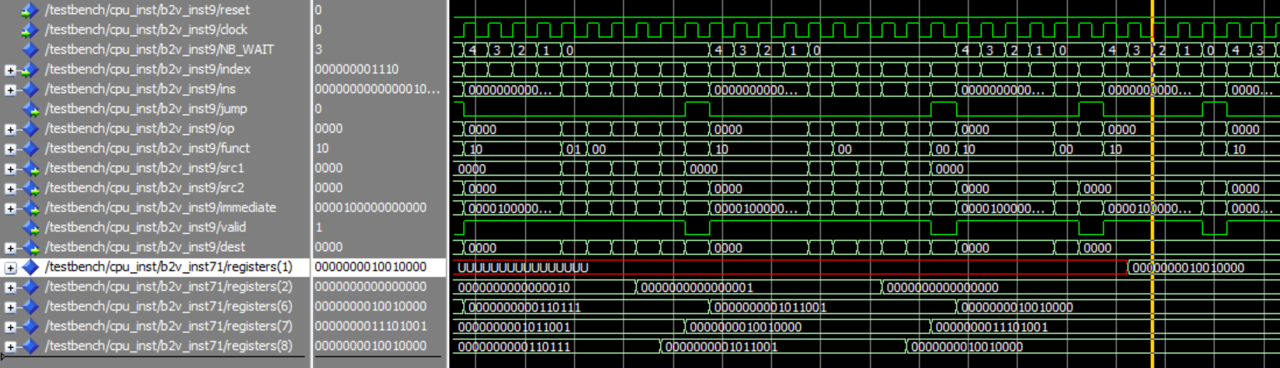
\includegraphics[width=\textwidth]{figures/simulation.png}
    \caption{Résultats de la simulation avec \texttt{fibo.out}}
    \label{fig:simulation}
\end{figure}

Avec le programme \texttt{fibo.out} (résultats en figure \ref{fig:simulation}),
l'évolution de \texttt{NB\_WAIT}, \texttt{index} et \texttt{ins} semble
confirmer la bonne gestion des sauts. De plus, la valeur finale stockée dans
\texttt{x1} est $0b10010000 = 144$. Or $F_{12} = 144$: on a bien le résultat
attendu ! \\

En revanche, cela ne prouve pas le bon fonctionnement du processeur, car
l'ensemble de ses fonctionnalités n'est pas exhaustivement testé par
\texttt{fibo.asb}. En particulier, la pile n'est pas utilisée.



% References

% \figureslist                    % list of figures
% \tableslist                     % list of tables
% \scriptslist                    % list of scripts
\bibliographyreferenceslist     % bibliography


% Appendices

\appendix
% \input{appendices/XXX.tex}

\end{document}
